% % % % % % % % % % % % % % % % % % % % % % % % % % % % % % % % % % % % % % % %
% LaTeX4EI Template for Cheat Sheets                                Version 1.0
%
% Authors: Markus Kaschke
% Contact: info@latex4ei.de
% Encode: UTF-8, tabwidth = 4, newline = LF
% % % % % % % % % % % % % % % % % % % % % % % % % % % % % % % % % % % % % % % %


% ======================================================================
% Document Settings
% ======================================================================

% possible options: color/nocolor, english/german, threecolumn
% defaults: color, english
\documentclass[english]{latex4ei/latex4ei_sheet}

% set document information
\title{NLASP}
\author{Markus Kaschke}					% optional, delete if unchanged
\myemail{info@latex4ei.de}			% optional, delete if unchanged
\mywebsite{www.latex4ei.de}			% optional, delete if unchanged


\let\T\relax
\DeclareMathOperator{\T}{\textsf{\textit{T}}}		% Zufallsvariable X
\DeclareMathOperator{\Bias}{Bias}		% Zufallsvariable X
\DeclareMathOperator{\argmax}{argmax}

\DeclareMathOperator{\rang}{rang}
\renewcommand{\vec}[1]{\underline{\boldsymbol{#1}}}
%\renewcommand{\vec}[1]{\boldsymbol{#1}}



\newcommand{\x}{\textit{x}}
\newcommand{\vx}{\underline{\textbf{\textit{x}}}}
\newcommand{\VX}{\underline{\textbf{\textit{X}}}}

\newcommand{\y}{\textit{y}}
\newcommand{\vy}{\underline{\textbf{\textit{y}}}}
\newcommand{\VY}{\underline{\textbf{\textit{Y}}}}


\newcommand{\VA}{\underline{\textit{A}}}
\newcommand{\A}{\textit{A}}
\newcommand{\va}{\underline{\textbf{\textit{a}}}}

\newcommand{\VB}{\underline{\textit{B}}}


% ======================================================================
% Begin
% ======================================================================
\begin{document}

\IfFileExists{git.id}{\input{git.id}}{}
\ifdefined\GitRevision\mydate{\GitNiceDate\ (git \GitRevision)}\fi
% Title
% ----------------------------------------------------------------------
\maketitle   % requires ./img/Logo.pdf

% Section
% ----------------------------------------------------------------------
\section{Math}
% ======================================================================

\begin{sectionbox}
    \begin{tabular}{@{}llll}
        $\pi \approx \num{3,14159}$ & $e \approx \num{2,71828}$ & $\sqrt{2} \approx \num{1,414}$ & $\sqrt{3} \approx \num{1,732}$ \\
    \end{tabular}

    \textbf{Binome, Trinome}\\
    $(a\pm b)^2 = a^2 \pm 2ab + b^2$ \hfill $a^2 - b^2 = (a-b)(a+b)$\\
    $(a \pm b)^3 = a^3 \pm 3a^2b + 3ab^2 \pm b^3$\\
    $(a+b+c)^2 = a^2 + b^2 + c^2 + 2ab + 2ac + 2bc$
    \\[0.5em]
    \textbf{Folgen und Reihen}\\
    $\underset{\text{Aritmetrische Summenformel}}{\sum \limits_{k=1}^{n} k = \frac{n (n+1)}{2}}$ \quad $\underset{\text{Geometrische Summenformel}}{\sum \limits_{k=0}^{n} q^k = \frac{1 - q^{n+1}}{1-q}}$ \quad $\underset{\text{Exponentialreihe}}{\sum\limits_{n = 0}^{\infty} \frac{\cx z^n}{n!} = e^{\cx z}}$\\
    \\[0.5em]
    \textbf{Mittelwerte} \quad ($\sum$ von $i$ bis $N$) \hfill {\small (Median: Mitte einer geordneten Liste)}\\
    \begin{tabular*}{\columnwidth}{@{\extracolsep\fill}l@{\quad\ $\ge$}l@{\quad\ $\ge$}l}
        $\underset{\text{Arithmetisches}}{\ol x_{\ir{ar}} = \frac{1}{N} \sum x_i}$ & $\underset{\text{Geometrisches Mittel}}{\ol x_{\ir{geo}} = \sqrt[N]{ \prod x_i }}$ & $\underset{\text{Harmonisches}}{\ol x_{\ir hm} = }\frac{N}{\sum \frac{1}{x_i}}$\\
    \end{tabular*}
    \\[0.5em]
    \textbf{Ungleichungen:} \hfill Bernoulli-Ungleichung:  $(1+x)^n \ge 1+nx$\\
    $\underset{\text{Dreiecksungleichung}}{\big|\! \abs{x}- \abs{y}\!\big| \le \abs{x \pm y} \le \abs{x} + \abs{y}}$ \hfill
    $\underset{\text{Cauchy-Schwarz-Ungleichung}}{\left| \vec x^\top \bdot \vec y \right| \le \| \vec x\| \cdot \| \vec y\|}$
    \\[0.5em]
    \textbf{Mengen:} De Morgan: $\overline{A \capdot B} = \overline{A} \cupplus \overline{B}$ \hfill $\overline{A \cupplus B} = \overline{A} \capdot \overline{B}$
\end{sectionbox}

\begin{sectionbox}
    \subsection[Exp. und Log.]{Exp. und Log.\ \ $e^x := \lim\limits_{n \rightarrow \infty} \left( 1 + \frac{x}{n} \right)^n \hfill e \approx 2,71828$}
    \begin{tabular*}{\columnwidth}{@{\extracolsep\fill}lll@{}}
        $a^x = e^{x \ln a}$ & $\log_a x = \frac{\ln x}{\ln a}$ & $\ln x \le x -1$\\
        $\ln(x^{a}) = a \ln(x)$ & $\ln(\frac{x}{a}) = \ln x - \ln a$ & $\log(1) = 0$\\
    \end{tabular*}
\end{sectionbox}


\begin{sectionbox}
    \subsection[Matrizen]{Matrizen $\ma A \in\mathbb{K}^{m \times n}$}
    $\ma A=(a_{ij}) \in \mathbb K^{m\times n}$ hat $m$ Zeilen (Index $i$) und $n$ Spalten (Index $j$)
    \begin{tabular*}{\columnwidth}{ll}
        $(\ma A + \ma B)^\top = \ma A^\top + \ma B^\top$ & $(\ma A \cdot \ma B)^\top = \ma B^\top \cdot \ma A^\top$\\
        ${(\ma A^\top)}^{-1} = {(\ma A^{-1})}^\top$ & $(\ma A \cdot \ma B)^{-1} = \ma B^{-1}\ma A^{-1}$
    \end{tabular*}
    $\dim \mathbb K = n = \rang\ma A + \dim\ker\ma A$ \qquad $\rang\ma A = \rang\ma A^\top$


    \subsubsection{Quadratische Matrizen $A \in \mathbb{K}^{n \times n}$}
    regulär/invertierbar/nicht-singulär $\Leftrightarrow \det (\ma A) \ne 0 \Leftrightarrow \rang\ma A = n$\\
    singulär/nicht-invertierbar $\Leftrightarrow \det (\ma A) = 0 \Leftrightarrow \rang\ma A \ne n$\\
    orthogonal $\Leftrightarrow \ma A^\top=\ma A^{-1} \Ra \det(\ma A) = \pm 1$\\
    symmetrisch: $\ma A=\ma A^\top$ \qquad schiefsymmetrisch: $\ma A=-\ma A^\top$
    %\item hermitsch: $\ma A=\overline{\ma A}^\top$, unitär:$\ma A^{-1} = \overline{\ma A}^\top$


    \subsubsection[Determinante]{Determinante von $\ma A\in \mathbb K^{n\times n}$: $\det(\ma A)=|\ma A|$}
    $\det\mat{ \ma A & \ma 0 \\ \ma C& \ma D }= \det\mat{ \ma A & \ma B \\ \ma 0 & \ma D } = \det(\ma A)\det(\ma D)$ \\
    \begin{tabular*}{\columnwidth}{@{\extracolsep\fill}ll}
        $\det(\ma A) = \det(\ma A^T)$ & $\det(\ma A^{-1}) = \det(\ma A)^{-1}$
    \end{tabular*}
    $\det(\ma A\ma B) = \det(\ma A)\det(\ma B) = \det(\ma B)\det(\ma A) = \det(\ma B\ma A)$\\
    Hat $\ma A$ 2 linear abhäng. Zeilen/Spalten $\Rightarrow |\ma A|=0$ \\

    \subsubsection{Eigenwerte (EW) $\lambda$ und Eigenvektoren (EV) $\underline v$}
    \begin{emphbox}
        \large $\ma A \vec v = \lambda \vec v$ \quad\ $\det \ma A = \prod \lambda_i$ \quad\ $\Sp \ma A = \sum a_{ii} = \sum \lambda_i$
    \end{emphbox}
    Eigenwerte: $\det(\ma A - \lambda \ma 1) = 0$ Eigenvektoren: $\ker(\ma A - \lambda_i \ma 1) = \vec v_i$\\
    EW von Dreieck/Diagonal Matrizen sind die Elem. der Hauptdiagonale.


    \subsubsection{Spezialfall $2 \times 2$ Matrix $A$}
    \parbox{3cm}{ $\det(\ma A) = ad-bc$ \\ $\Sp(\ma A) = a+d$ } $\mat{a & b\\ c & d}^{-1} = \frac{1}{\det \ma A} \mat{d & -b\\ -c& a}$\\
    $\lambda_{1/2} = \frac{\Sp \ma A}{2} \pm \sqrt{ \left( \frac{\mathrm{sp} \ma A}{2} \right)^2 - \det \ma A }$

    \subsubsection{Differentiation}
    $\frac{\partial \vec x^\top \vec y}{\partial \vec x} = \frac{\partial \vec y^\top \vec x}{\partial \vec x} = \vec y$\qquad
    $\frac{\partial \vec x^\top \ma A \vec x}{\partial \vec x} = (\ma A + \ma A^\top)\vec x$ \\
    $\frac{\partial \vec x^\top \ma A \vec y}{\partial \ma A} = \vec x \vec y^\top$ \qquad $\frac{\partial \det( \ma B \ma A \ma C )}{\partial \ma A} = \det(\ma B \ma A \ma C) \left( \ma A^{-1} \right)^\top$
\end{sectionbox}



\begin{sectionbox}
    \subsubsection{Ableitungsregeln ($\forall \lambda, \mu \in \mathbb R$)}
    \begin{tabular}{@{}l@{\quad}ll@{}}
        Linearität: & $(\lambda f + \mu g)' (x) = \lambda f'(x) + \mu g'(x_0)$                                                                             \\
        Produkt:    & $(f \cdot g)'(x) = f'(x) g(x) + f(x) g'(x)$                                                                                          \\
        Quotient:   & $\left(\frac{f}{g}\right)' (x) = \frac{g(x)f'(x) -f(x) g'(x)}{g(x)^2}$ \quad $\left(\frac{\text{NAZ}-\text{ZAN}}{\text{N}^2}\right)$ \\
        Kettenregel & $\left( f\bigl(g(x)\bigr) \right)' = f'\bigl(g(x)\bigr) g'(x)$                                                                       \\
    \end{tabular}
\end{sectionbox}

\begin{sectionbox}
    \subsection{Integrale $\int e^x\mathrm dx = e^x = (e^x)'$}
    %$\int_a^b f(x) \mathrm dx = F(b) - F(a)$\\
    \begin{tabular*}{\columnwidth}{ll}
        Partielle Integration: & $\int uw'=uw-\int u'w$\\
        Substitution: & $\int f(g(x)) g'(x)\diff x=\int f(t)\diff t$
    \end{tabular*}
    \begin{tablebox}{@{\hspace{5mm}}c@{\extracolsep\fill}c@{\extracolsep\fill}c@{\hspace{5mm}}}
        $F(x) - C$ & $f(x)$ & $f'(x)$ \\ \cmrule
        $\frac{1}{q+1}x^{q+1}$ & $x^q$ & $qx^{q-1}$ \\[1em]
        \raisebox{-0.2em}{$\frac{2\sqrt{ax^3}}{3}$} & $\sqrt{ax}$ & \raisebox{0.2em}{$\frac{a}{2\sqrt{ax}}$}\\
        $x\ln(ax) -x$ & $\ln(ax)$ & $\textstyle \frac{1}{x}$\\
        $\frac{1}{a^2} e^{ax}(ax- 1)$ & $x \cdot e^{ax}$ & $e^{ax}(ax+1)$ \\
        $\frac{a^x}{\ln(a)}$ & $a^x$ & $a^x \ln(a)$ \\
        $-\cos(x)$ & $\sin(x)$ & $\cos(x)$\\
        $\cosh(x)$ & $\sinh(x)$ & $\cosh(x)$\\
        $-\ln |\cos(x)|$ & $\tan(x)$ & $\frac{1}{\cos^2(x)}$ \\
    \end{tablebox}

    \begin{tabular*}{\columnwidth}{ll}
        \multicolumn{2}{c}{$\int e^{at} \sin(bt) \diff t = e^{at} \frac{a \sin(bt) + b \cos(bt)}{a^2 + b^2}$}\\
        $\int \frac{\diff t}{\sqrt{at+b}} = \frac{2 \sqrt{at+b}}{a}$ & $\int t^2 e^{at} \diff t = \frac{(ax-1)^2+1}{a^3} e^{at}$\\
        $\int t e^{at} \diff t = \frac{at-1}{a^2} e^{at}$ & $\int x e^{ax^2} \diff x = \frac{1}{2a} e^{ax^2}$\\
    \end{tabular*}

    \subsubsection{Volumen und Oberfläche von Rotationskörpern um $x$-Achse}
    $V = \pi \int_a^b f(x)^2 \mathrm dx$ \qquad \quad $O = 2 \pi \int_a^b f(x) \sqrt{1 + f'(x)^2} \mathrm dx$
\end{sectionbox}


% Section
% ----------------------------------------------------------------------
\section{Floating-Point Arithmetics}
% ======================================================================


\begin{sectionbox}
    \subsection{IEEE 754}
    Representation of real number $x\in\mathbb{R}$:\\

    $x = (-1)^s(1+m2^{-t})2^{e-\beta}$\\

    \begin{tabular}{lll}
        Single Precision & 1.8.23  \\
        Double Precision & 1.11.52 \\
    \end{tabular}

    \begin{tabular}{ll}
        Largest finite number    & $(2-2^{-t})2^{1-\frac{e_{max}}{2}}$ \\
        Smallest non zero Number & $2^{1-\frac{e_{max}-1}{2}}$
    \end{tabular}\\

    \textbf{Accuracy}:\\

    $\frac{\left|x_2 - x_1\right|}{\left|x_1\right|} \leq 2^{-t}$\\

    \textbf{Machine Epsilon $\epsilon_M$}\\

    $\textit{fl}(x) = x(1+\epsilon)$ \hfil $\textit{fl}(x) = \frac{x}{1+\epsilon}$\\
    with different $\epsilon$.\\

    Maximum error is half the precision given by \\
    Machine Epsilon: $\epsilon_M = 2^{-t-1}$.

    \textbf{Worst case error}\\
    $\rho = r(1+\theta_n)$ with $|\theta_n| \leq \frac{n\epsilon_M}{1-\frac{n}{2}\epsilon_M}$.\\
    The number of operations is given by $n$.\\

    A more general formulation is:\\
    $\rho = r\Pi_{i=1}^{n} (1+\epsilon_i)^{\eta_i}$ with $\eta_i \in \{-1;+1\}$ this results in:\\
    $\rho=r(1+\theta_n)$ with $|\theta_n| \leq \gamma_n$ and $\gamma_n = \frac{n\epsilon_M}{1-\frac{n}{2}\epsilon_M}$


\end{sectionbox}
\begin{sectionbox}

    \subsection{Complex Floating Point Arithmetic}
    The error in complex floating point operations can also be represented with:\\
    $x\odot y= (x\circ y)(1+\epsilon)$\\

    with $|\epsilon|\leq \alpha \epsilon_M$. The alpha coefficients are given in the table below:\\

    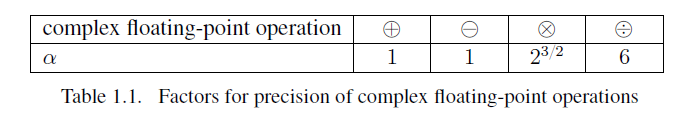
\includegraphics[width=\textwidth]{img/cplx_fl_op.png}

\end{sectionbox}
\section{Linear Algebra}
\begin{sectionbox}
    \subsection{SVD}
    A matrix is unitary if: $\mathbf{U}^H\mathbf{U}=\mathbf{U}\mathbf{U}^H =\mathbf{I}$\\

    The singular decomposition (SVD) of the matrix $\mathbf{A}\in\mathbb{C}^{mxn}$ reads as:\\
    $\mathbf{A} = \mathbf{U}\mathbf{\Sigma}\mathbf{V}^H$ where:\\
    $\mathbf{U}$ and $\mathbf{V}$ are unitary and $\mathbf{\Sigma}\in\mathbb{C}^{mxn}$ is diagonal.\\

    $\mathbf{\Sigma}_0 = \text{diag}(\sigma_1, \sigma_2, ...,\sigma_{\text{min}(m,n)})$

    $\mathbf{\Sigma} = \begin{cases}
            \mathbf{\Sigma}_0, \text{for } m=n                                       \\
            [\mathbf{\Sigma}_0, \mathbf{0}], \text{for } m < n \text{ (wide matrix)} \\
            \begin{bmatrix}
                \mathbf{\Sigma}_0, \\
                \mathbf{0}
            \end{bmatrix}, \text{for } m > n \text{ (tall matrix)}
        \end{cases}$\\

    The \textbf{SVD} can also be represented in the following form:\\

    $\mathbf{A} = \sum_{i=1}^{\text{min(m,n)}} \sigma_i \mathbf{u}_i\mathbf{v}_i^H$\\

    with\\
    $\mathbf{U} = [\mathbf{u}_1,\mathbf{u}_2,...\mathbf{u}_m] \in\mathbb{C}^{mxm}$\\
    $\mathbf{V} = [\mathbf{v}_1, \mathbf{v}_2, ...\mathbf{v}_n] \in\mathbb{C}^{nxn}$\\

    The rank of $r=rank(\mathbf{A})$ is given by the number of \textbf{non zero} singular values $\sigma_i>0$\\
    $range(\mathbf{A}) = span(\mathbf{u}_1,...\mathbf{u}_r)$\\
    $null(\mathbf{A}) = span(\mathbf{v}_{r+1},  ...\mathbf{v}_n)$\\

    Removing the singular values that are zero $\sigma_{r+1}=...=\sigma_{n}=0$ the reduced SVD can be expressed with:\\

    $\mathbf{A} = \mathbf{U}_{red}\mathbf{\Sigma}_{red}\mathbf{V}^H_{red}$\\
    with\\
    $\mathbf{\Sigma}_{red} = \text{diag}(\sigma_1, ...\sigma_r)$,
    $\mathbf{U}_{red} = [\mathbf{u}_1, ...\mathbf{u}_r]$ and\\
    $\mathbf{V}_{red} = [\mathbf{v}_1, ...\mathbf{v}_r]$\\

    \textbf{Gram Matrix}\\

    $\mathbf{B} = \mathbf{A}\mathbf{A}^H$ is Hermitian by definition. It's SVD reads as:\\

    $\mathbf{B} = \mathbf{U}_{red}\mathbf{\Sigma}_{red}\mathbf{U}_{red}^H$\\
    A similar discussion is possible for $\mathbf{C} = \mathbf{A}^H\mathbf{A}$:\\

    $\mathbf{C}=\mathbf{A}^H\mathbf{A} = \mathbf{V}_{red}\mathbf{\Sigma}_{red}\mathbf{V}^H_{red}$\\

    Both decompositions are like the (reduced) EVD.\\
    When computing the Gram matrix $\mathbf{A}^\text{H}\mathbf{A}$, every element is equal to the inner product of the two corresponding columns of $\mathbf{A}$. Let $\mathbf{a}_i$ denote the $i$-th column of $\mathbf{A}$. Then, the $i,j$-element of the Gram matrix can be written as
    $$[\mathbf{A}^\text{H}\mathbf{A}]_{ij} = \mathbf{a}_i^\text{H}\mathbf{a}_j$$\\
    Only the upper triangular part of $\mathbf{A}^\text{H}\mathbf{A}$ must be computed due to the Hermitian structure of $\mathbf{A}^\text{H}\mathbf{A}$. The lower triangular are simply the complex conjugate of the corresponding elements of the upper triangular.\\
    \textbf{Operation Count Gram Matrix}: \#FLOPS $=\mathcal{O}(mn^2)$
\end{sectionbox}
\begin{sectionbox}
    \subsection{Projectors}
    Projectors are idempotent matrices. $\mathbf{P} \in \mathbb{C}^{mxm}$ is a projector if:\\
    $$\mathbf{P}^2 = \mathbf{P}$$

    \textbf{Orthogonal projectors} are additionally Hermitian. Therefore:\\
    $$\mathbf{P}^2 = \mathbf{P} \text{ and } \mathbf{P}^H=\mathbf{P}$$

    is a orthogonal projector.\\

    The orthogonal complement of a projector $\mathbf{P}$ is defined as:\\
    $\mathcal{S}_P^\perp = \{\mathbf{v}: (\mathbf{I}-\mathbf{P})\mathbf{v}=\mathbf{v}\}$\\

    The eigenvalues of a projector are out of the set $\lambda_i\in\{1;0\}$. And therefore:

    $$\mathbf{P} = \mathbf{U}\text{diag}(1,...,1,0,...0)\mathbf{U}^H$$

    with reads in the reduced form:
    $$\mathbf{P} = \mathbf{U}_{red}\mathbf{U}_{red}^H = \sum_{i=1}^{r}\mathbf{u}_i\mathbf{u}_i^H$$
    with $\mathbf{U}_{red} = [\mathbf{u}_1,...,\mathbf{u}_r]$.
    Furthermore it can be concluded that:

    $$rank(\mathbf{P}) = tr(\mathbf{P}) =r$$.
\end{sectionbox}
\begin{sectionbox}
    \subsubsection{Projectors of vectors}
    We can construct a projector of a vector $\mathbf{a}$ according to:
    $$\mathbf{P}_a = \frac{\mathbf{a}\mathbf{a}^H}{\parallel\mathbf{a}\parallel^2_2}$$

    The projector onto the orthogonal complement is given by:
    $$\mathbf{P}^\perp_\mathbf{a} = \mathbf{I}-\mathbf{P}_a = \mathbf{I} - \frac{\mathbf{a}\mathbf{a}^H}{\parallel\mathbf{a}\parallel^2_2}$$
    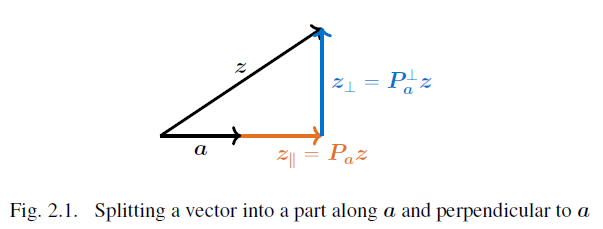
\includegraphics[width=\textwidth]{img/vector_decomp.png}

    Given orthogonal vectors $\mathbf{a}_1, ... \mathbf{a}_n$ we can perform multiple projections onto the orthogonal complement via:\\
    $$\prod_{i=1}^n \mathbf{P}_{\mathbf{a}_i}^\perp = \mathbf{I} - \sum_{i=1}^{n}\frac{\mathbf{a}_i\mathbf{a}_i^H}{\parallel\mathbf{a}_i\parallel^2_2}$$
\end{sectionbox}
\begin{sectionbox}
    \subsection{Matrix and Vector norms}
    \textbf{Vector norms}:\\

    \begin{tabular*}{\columnwidth}{ll}
        p-norm: & $\parallel\mathbf{x}\parallel_p = \sqrt[p]{\sum_{i=1}^{n} |x_i|^p}$\\
        1-norm: & $\parallel\mathbf{x}\parallel_1 = \sum_{i=1}^{n} |x_i|$\\
        2-norm: & $\parallel\mathbf{x}\parallel_2 = \sqrt{\sum_{i=1}^{n} |x_i|^2}$\\
        $\infty$-norm & $\parallel\mathbf{x}\parallel_\infty = \max_{i\in\{1,...,n\}} |x_i|$\\
    \end{tabular*}\\

    \textbf{Matrix norms}:\\
    $\parallel \mathbf{A}\parallel \leq \parallel \mathbf{A}\parallel \parallel\mathbf{B}\parallel$
    The columnwise vectorization of $\mathbf{A}$ reads as:\\
    $\text{vec}(\mathbf{A}) = [\mathbf{a}_1^T, ...,\mathbf{a}_n^T]^T\in\mathbb{C}^{mxn}$\\

    $$\parallel\mathbf{A}\parallel_F = \parallel vec(A)\parallel_2 = \sqrt{\sum_{i=1}^{m}\sum_{j=1}^{n} |a_{ij}|^2}$$
\end{sectionbox}
\begin{sectionbox}
    \subsection{Householder Reflection}
    With the Householder Reflection we want remove all elements of a vector except the first one. Give a vector $\mathbf{x}$:\\
    $\mathbf{x} = \begin{bmatrix}
            x_1 \\
            \mathbf{x}_2
        \end{bmatrix}\in\mathbb{C}^m$\\

    With the unitary matrix $\mathbf{F}\in\mathbb{C}^{mxm}$ ($\mathbf{F}^H\mathbf{F}=\mathbf{F}\mathbf{F}^H = \mathbf{I}$)we want to achieve the following:\\
    $$\mathbf{F}\mathbf{x} = \begin{bmatrix}
            \alpha \\
            0      \\
            \vdots \\
            0
        \end{bmatrix} = \alpha \mathbf{e}_1$$\\
    It follows: $\parallel\mathbf{F}\mathbf{x}\parallel_2^2 = \mathbf{x}^H\mathbf{F}^H\mathbf{F}\mathbf{x} = \parallel \mathbf{x}\parallel_2^2$ and therefore:\\
    $|\alpha| = \parallel \mathbf{x}\parallel_2^2$\\
    The overall goal is to find the matrix $\mathbf{F}$ that achieves:
    $$\mathbf{F}\mathbf{x} = \begin{bmatrix}
            \parallel \mathbf{x}\parallel_2 e^{j\phi} \\
            0                                         \\
            \vdots                                    \\
            0
        \end{bmatrix} = \parallel \mathbf{x}\parallel_2 e^{j\phi} \mathbf{e}_1$$\\
    We want to find the vector\\

    $\mathbf{v} = \parallel\mathbf{x}\parallel_2 e^{j\phi}\mathbf{e}_1 - \mathbf{x}$\\

    The vectors $\mathbf{x}$, $\mathbf{v}$ and $\parallel\mathbf{x}\parallel_2 e^{j\phi}\mathbf{e}_1$ form an isosceles triangle. The height vector is given by the projection onto the orthogonal complement of $\mathbf{v}$:

    $\mathbf{h} = \mathbf{P}^\perp_\mathbf{v}\mathbf{x} = (\mathbf{I} - \mathbf{P}_\mathbf{v})\mathbf{x} = \mathbf{x} - \frac{\mathbf{v}\mathbf{v}^H}{\parallel\mathbf{v}\parallel_2^2} \mathbf{x}$

    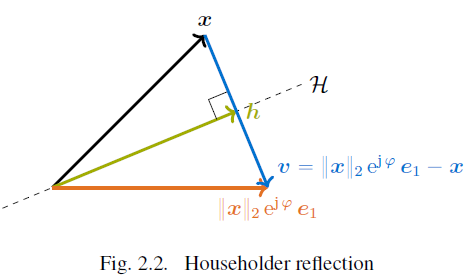
\includegraphics[width=\textwidth]{img/householder.png}

    The matrix $\mathbf{F}$ is given by:
    $$\mathbf{F} = \mathbf{I} - 2\frac{\mathbf{v}\mathbf{v}^H}{\parallel\mathbf{v}\parallel_2^2}$$

    Decomposing the Householder reflector into it's EVD leads to:

    $$[\mathbf{w}, \mathbf{W}_\perp]\text{diag}(-1,1,...,1)[\mathbf{w},\mathbf{W}_\perp]^H$$\\

    where $\mathbf{w} = \frac{\mathbf{v}}{\parallel \mathbf{v}\parallel_2}$ and $\mathbf{P}_\mathbf{v}^\perp = \mathbf{W}_perp\mathbf{W}_\perp^H$\\
    Only $\lambda_1=-1$ of $\mathbf{F}$ all other eigenvalues are $\lambda_i=1$.
\end{sectionbox}

\begin{sectionbox}
    \subsubsection{Choice of Phase after Reflection}

    A possible choice is: $\phi=0$ such that $\alpha$ is positive-real.
    An other goal is to make $\mathbf{v}$ as long as possible therefore:
    $$\phi_{opt} = \text{argmax}_{\phi} = \parallel \mathbf{v}\parallel_2^2$$
    with $\mathbf{x} = [x_1, \mathbf{x}_2^T]^T$ and \\
    $\mathbf{v} = \parallel \mathbf{x}\parallel_2 e^{j\phi}\mathbf{e}_1 - \mathbf{x}$ the objective function can be expressed as
    $$\parallel \mathbf{v} \parallel_2^2 = |e^{j\phi}\parallel\mathbf{x}\parallel_2 - x_1|^2 + \parallel \mathbf{x}_2 \parallel_2^2$$
    As the second term is independent of $\phi$, the first term must be maximized. To this end, it is necessary to choose $\phi_{opt}=\psi+\pi$ for $x_1 = |x_1|e^{j\psi}$, resulting in
    $$\mathbf{v} = \begin{bmatrix}
            -(\parallel\mathbf{x}\parallel_2 + |x_1|)e^{j\psi} \\
            -\mathbf{x}_2
        \end{bmatrix}$$
    The maximum objective function is:
    $$\parallel\mathbf{v}_{opt}\parallel_2^2 = 2\parallel\mathbf{x}_2\parallel_2^2 + 2|x_1|\parallel\mathbf{x}\parallel_2$$

\end{sectionbox}
\section{QR Decomposition}
\begin{sectionbox}
    For a full-rank and tall matrix $\mathbf{A} = [\mathbf{a}_1, ...,\mathbf{a}_n] \in \mathbb{C}^{mxn}$ with $m\gg n$ the QR decomposition reads as:
    $$\mathbf{A} = \mathbf{Q}\mathbf{R}$$
    where $\mathbf{Q}\in\mathbb{C}^{mxm}$ is unitary and
    $$\mathbf{R}=\begin{bmatrix}
            \mathbf{R}_{red} \\
            \mathbf{0}
        \end{bmatrix} \in \mathbb{C}^{mxn}$$
    with
    $$\mathbf{R}_{red} = \begin{bmatrix}
            r_{11} & r_{12} & \cdots & r_{1n} \\
            0      & r_{22} & \cdots & r_{2n} \\
            0      & 0      & \ddots & \vdots \\
            0      & \cdots & r_{nn}
        \end{bmatrix} \in \mathbb{C}^{nxn}$$

    with ($\nu \leq n$):\\
    $span(\mathbf{a}_1, ...,\mathbf{a}_\nu) = span(\mathbf{q}_1, ...,\mathbf{q}_\nu)$\\
    which results in:\\
    $range(\mathbf{A}) = span(\mathbf{a}_1, ...,\mathbf{a}_n) = span(\mathbf{q}_1, ...,\mathbf{q}_n) = range(\mathbf{Q}_{red})$\\
    $\mathbf{Q}_{red}$ is an orthonormal basis for the range space of $\mathbf{A}$. \\

    $\mathbf{Q}_{red} = [\mathbf{q}_1, ...,\mathbf{q}_n]\in \mathbb{C}^{mxn}$

    $\mathbf{Q}^\perp_{red} = [\mathbf{q}_{n+1}, ... ,\mathbf{q}_m] \in \mathbb{C}^{mxm-n}$\\
    It follows from
    $\mathbf{Q} = [\mathbf{Q}_{red},\mathbf{Q}_{red}^\perp]$ that\\
    $$\mathbf{I} = \mathbf{Q}^H\mathbf{Q} = $$
    $$\begin{bmatrix}
            \mathbf{Q}_{red}^H \\
            \mathbf{Q}_{red}^{\perp,H}
        \end{bmatrix} \cdot [\mathbf{Q}_{red}, \mathbf{Q}_{red}^\perp] = \begin{bmatrix}
            \mathbf{Q}_{red}^H\mathbf{Q}_{red}         & \mathbf{Q}_{red}^H\mathbf{Q}_{red}^\perp         \\
            \mathbf{Q}_{red}^{\perp,H}\mathbf{Q}_{red} & \mathbf{Q}_{red}^{\perp,H}\mathbf{Q}_{red}^\perp
        \end{bmatrix}$$\\

    Therefor: $\mathbf{Q}_{red}^H\mathbf{Q}_{red}^\perp = 0$. Consequently the space spanned by the columns of $\mathbf{Q}_{red}^\perp$ is perpendicular to $range(\mathbf{Q}_{red})$. In other words:
    $$null(\mathbf{A}^H) = range(\mathbf{Q}_{red}^\perp)$$\\
    that is, the matrix $\mathbf{Q}_{red}^\perp$ is a basis for the left nullspace of $\mathbf{A}$.

\end{sectionbox}
\begin{sectionbox}
    \subsection{Operation Count of basic operations}
    \begin{tablebox}{@{\hspace{5mm}}c@{\extracolsep\fill}c@{\extracolsep\fill}c@{\hspace{5mm}}}
        $f$ & Mult.+Sum. & \#FLOPS \\ \cmrule
        $\mathbf{a}^H\mathbf{b} = \sum_{i=1}^{m}a_i^*b_i$ & $m$+$m-1$ & $2m-1$ \\
        $\parallel\mathbf{a}\parallel_2 = \sqrt{\sum_{i=1}^{m} a_i^*a_i}$ & $m+m-1+1$ & $2m$\\
        $\gamma \mathbf{a}$ & $m$ & $m$\\
        $\mathbf{a}\pm\mathbf{b}$ & $m$ & $m$

    \end{tablebox}



\end{sectionbox}
\begin{sectionbox}
    \subsection{Classical Gram-Schmidt Orthogonalization}
    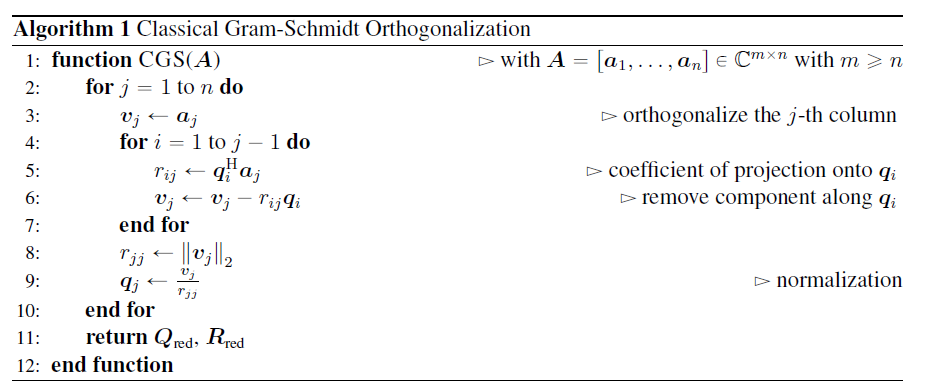
\includegraphics[width=\textwidth]{img/classic_gram_schmidt.png}

\end{sectionbox}

\begin{sectionbox}
    \subsection{Modified Gram-Schmidt Orthogonalization}
    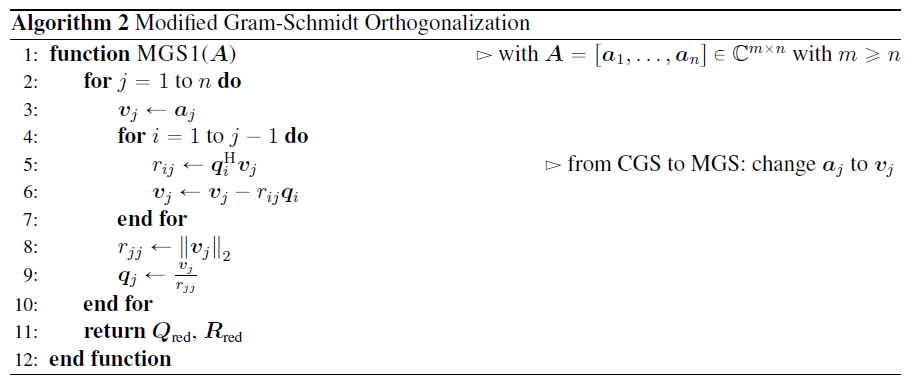
\includegraphics[width=\textwidth]{img/modified_gram_schmidt}

    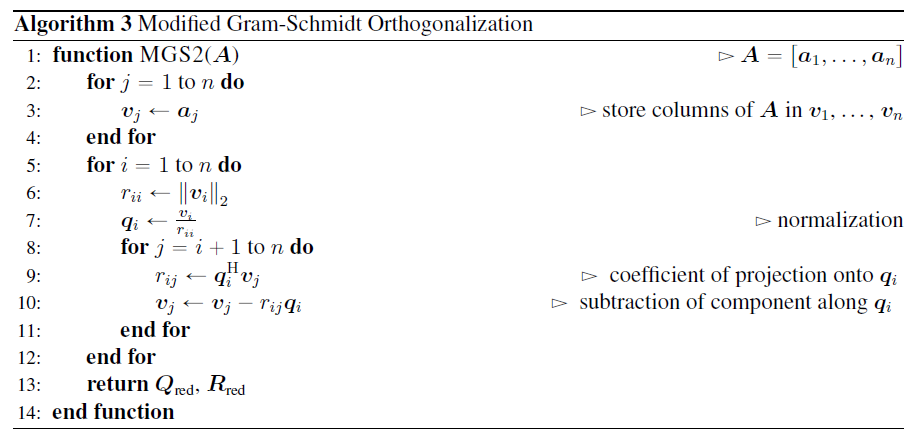
\includegraphics[width=\textwidth]{img/classic_gram_schmidt2.png}

    \textbf{Operation Count}: \#FLOPS $=\mathcal{O}(2mn^2)$
\end{sectionbox}
\begin{sectionbox}
    \subsection{Househodler QR Decomposition}

    With the Householder reflector $\mathbf{Q}_1 = \mathbf{F}_1$ the first column of matrix $\mathbf{A}$ is transformed as follows
    $$\mathbf{Q}_1 \mathbf{A} = \begin{bmatrix}
            \times & \times & \times \\
            0      & \times & \times \\
            0      & \times & \times \\
            0      & \times & \times \\
            0      & \times & \times
        \end{bmatrix}$$
    In the next step we apply the matrix $\mathbf{Q}_2$ which inherits a Householder reflector $\mathbf{F}_2\in\mathbb{C}^{m-1\times m-1}$
    $$\mathbf{Q}_2 = \begin{bmatrix}
            1          & \mathbf{0}^T \\
            \mathbf{0} & \mathbf{F}_2
        \end{bmatrix} \in \mathbb{C}^{m \times m}$$
    After that the matrix $\mathbf{Q}_2\mathbf{Q}_1\mathbf{A}$ looks like this
\end{sectionbox}
\begin{sectionbox}
    $$\mathbf{Q}_2\mathbf{Q}_1 \mathbf{A} = \begin{bmatrix}
            \times & \times & \times \\
            0      & \times & \times \\
            0      & 0      & \times \\
            0      & 0      & \times \\
            0      & 0      & \times
        \end{bmatrix}$$
    The unitary rotation matrix $\mathbf{Q}$ at step $i\in[1,...,n]$ is given by
    $$\mathbf{Q}_i = \begin{bmatrix}
            \mathbf{I}_{i-1} & \mathbf{0}   \\
            \mathbf{0}       & \mathbf{F}_i
        \end{bmatrix}\in\mathbb{C}^{m\times m}$$
    with $\mathbf{F}_i = \mathbf{I}-2\frac{\mathbf{v_i}\mathbf{v_i}^H}{\parallel \mathbf{v}\parallel_2^2} \in \mathbb{C}^{m-i+1 \times m-i+1}$\\

    After rotating all $n$ columns of $\mathbf{A}$ we generate the QR decomposition with

    $\mathbf{A} = \mathbf{Q}_1^H\mathbf{Q}_2^H\cdots\mathbf{Q}_n^H \mathbf{R} = \mathbf{Q}\mathbf{R}$\\

    $\mathbf{R} \in \mathbb{C}^{mxn}$\\
    Furthermore it holds\\
    $\mathbf{Q} = \mathbf{Q}_1^H\mathbf{Q}_2^H\cdots\mathbf{Q}_n^H = \mathbf{Q}_1\mathbf{Q}_2\cdots\mathbf{Q}_n$
    since $\mathbf{Q}_i$ is Hermitian.

\end{sectionbox}

\begin{sectionbox}
    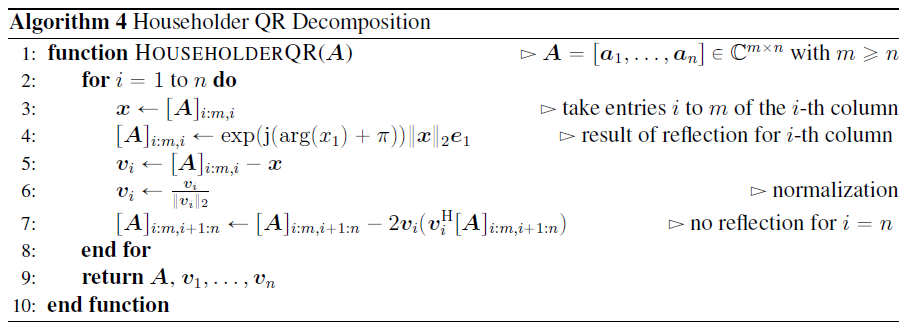
\includegraphics[width=\textwidth]{img/householder_QR.png}
    \textbf{Operation Count Algorithm $4$}: \#FLOPS $=\mathcal{O}(2mn^2 - \frac{2}{3}n^3)$
\end{sectionbox}
\begin{sectionbox}

    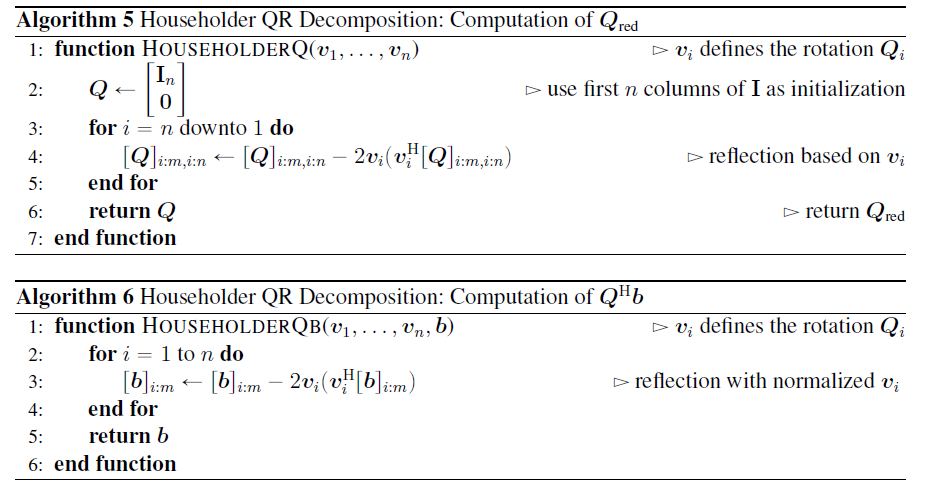
\includegraphics[width=\textwidth]{img/householder_QR_further.png}\\

    \textbf{Operation Count Algorithm $5$}: \#FLOPS $=\mathcal{O}(2mn^2-\frac{2}{3}n^3)$\\

    \textbf{Operation Count Algorithm $6$}: \#FLOPS $=\mathcal{O}(4mn-2n^2)$\\

    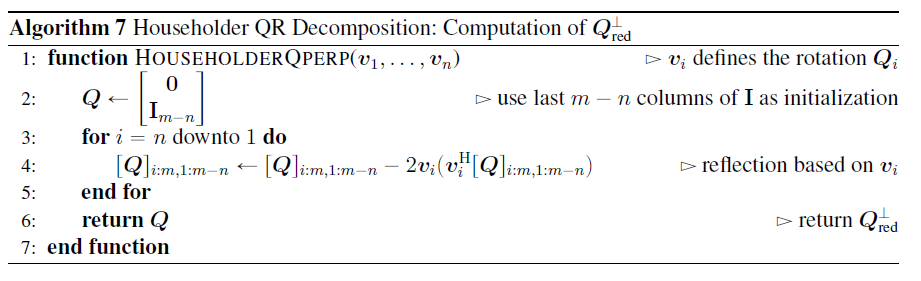
\includegraphics[width=\textwidth]{img/householder_QR_Qperp.png}\\

    \textbf{Operation Count Algorithm $7$}: \#FLOPS $=\mathcal{O}(4m^2n+2n^3-6mn^2)$\\
    If $m=n$ the number of FLOPS for Algorithm $7$ is zero, because the partition $\mathbf{Q}_red^\perp$ does not exist in this case.
\end{sectionbox}
\begin{sectionbox}
    \subsubsection{Householder for null($\mathbf{A}^H$)}

    In the case, that a basis for the nullspace $\mathbf{A}^H$, i.e., the orthogonal complement of $range(A)$ must be found Algorithm $7$ can be employed. null$(\mathbf{A}^H)=$range$(\mathbf{Q}_{red}^H)$

    $$\mathbf{Q} = [\mathbf{Q}_{red}, \mathbf{Q}_{red}^\perp]$$

\end{sectionbox}
\section{Back Substitution}
\begin{sectionbox}
    Solving an equation system with an upper triangular $\mathbf{R}$\\
    $\mathbf{R}\mathbf{x} = \mathbf{b}$\\
    can be solved with Algorithm $8$.


    $$\mathbf{R}= \begin{bmatrix}
            r_{11} & r_{12} & \cdots r_{1n}   \\
            0      & r_{22} &                 \\
                   & \ddots & \vdots          \\
                   &        & r_{nn}        &
        \end{bmatrix}\in\mathbb{C}^{n\times n}$$\\

    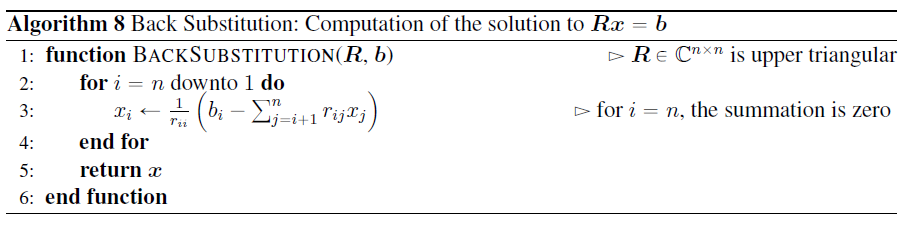
\includegraphics[width=\textwidth]{img/algo8_backsub.png}\\
    \textbf{Operation Count Algorithm $8$}: \#FLOPS $=\mathcal{O}(n^2)$\\
\end{sectionbox}

\begin{sectionbox}
    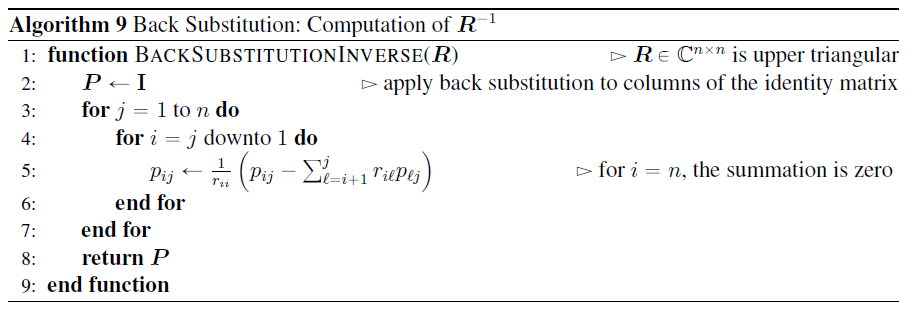
\includegraphics[width=\textwidth]{img/algo9_R_inverse.png}\\
    \textbf{Operation Count Algorithm $9$}: \#FLOPS $=\mathcal{O}(\frac{1}{3}n^3)$\\

    \#FLOPS$=\sum_{j=1}^{n}\sum_{i=1}^{j}(2j-2i+1)$\\
    $=\sum_{j=1}^{n}[2j^2-j(j+1)+j] = \frac{(2n+1)(n+1)n}{6}$
\end{sectionbox}

\section{Least Squares}
\begin{sectionbox}
    \subsection{Least Square for Full-Rank Matrix}
    $\mathbf{A}\mathbf{x} = \mathbf{b}$ with $\mathbf{A}\in\mathbb{C}^{m\times n}$ and $m\geq n$.
    For tall $\mathbf{A}\in\mathbb{C}^{m\times n}$ with $m>$ no solution exists in general, except $b\in$range$(\mathbf{A})$.

    For a square and invertible $\mathbf{A}$ the solution

    The Least Square solution is given by the normal equation:
    $$\mathbf{A}^H\mathbf{A}\mathbf{x}_{\text{LS}} = \mathbf{A}^H\mathbf{b}$$
    $$\mathbf{x}_{\text{LS}} = (\mathbf{A}^H\mathbf{A})^{-1}\mathbf{A}^H\mathbf{b}$$
    The pseudoinverse of $\mathbf{A}$: \quad $\mathbf{A}^\dagger = (\mathbf{A}^H\mathbf{A})^{-1}\mathbf{A}^H\mathbf{b}$

    \subsection{Least Square with Cholesky}
    We need to compute the Gram matrix: $\mathbf{A}^\text{H}\mathbf{A} = \mathbf{L}\mathbf{D}\mathbf{L}^\text{H}$.

    $$\mathbf{L}\mathbf{D}\mathbf{L}^\text{H} \mathbf{x}_{\text{LS}} = \mathbf{A}^\text{H}\mathbf{b}$$

    Due to $\mathbf{L}$ being lower triangular we need two times backsubstitution.

    The condition number with Cholesky increases because if we compute the Gram matrix it holds:
    $$\kappa (\mathbf{A}^H\mathbf{A}) = \kappa^2 (\mathbf{A})$$
    The condition number of the Gram matrix of $\mathbf{A}$ is the square of the original condition number $\kappa$.

\end{sectionbox}
\begin{sectionbox}
    \subsection{Least Square with QR}
    Using the decomposition $\mathbf{A} = \mathbf{Q}_{\text{red}}\mathbf{R}_{\text{red}}$
    We obtain the solution
    $$\mathbf{A}^\dagger = \mathbf{R}^{-1}_{\text{red}}\mathbf{Q}^\text{H}_{\text{red}}$$
    $$\mathbf{x}_{\text{LS}}=\mathbf{A}^\dagger \mathbf{b}$$
    Where $\mathbf{R}^{-1}_{\text{red}}$ describes a backsubstitution.
    Therefore we need to compute $\mathbf{Q}^\text{H}\mathbf{b}$ and then employ a backsubstitution on this result.
    QR decomposition and Cholesky have the same order of complexity if $m=n$.
\end{sectionbox}

\begin{sectionbox}
    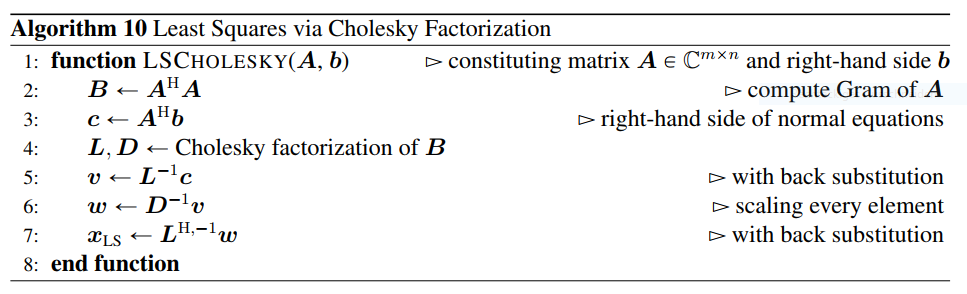
\includegraphics[width=\textwidth]{img/algo10_ls_with_cholesky.png}\\
    \textbf{Operation Count Algorithm $10$}: \#FLOPS $=\mathcal{O}(mn^2+\frac{1}{3}n^3)$\\
    Computing the Gram matrix and Cholesky factorization is dominant. In total we have:
    $\mathcal{O}(mn^2 + 2mn + \frac{1}{3}n^3 + 2n^2+n)$
\end{sectionbox}

\begin{sectionbox}
    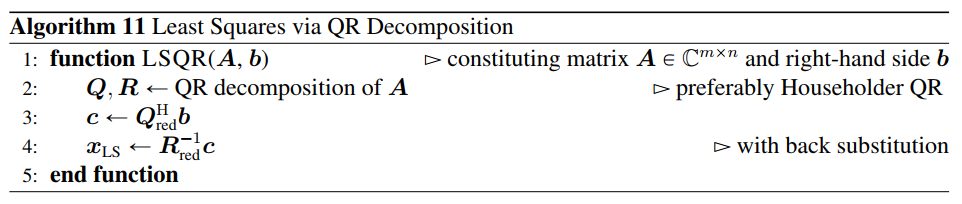
\includegraphics[width=\textwidth]{img/algo11_ls_with_QR.png}\\
    \textbf{Operation Count Algorithm $11$}: \#FLOPS $=\mathcal{O}(2mn^2-\frac{2}{3}n^3)$\\
    The complexity analysis assumes that we used Householder QR decomposition.
\end{sectionbox}
\begin{sectionbox}
    \subsection{Least Squares with SVD}
    We decompose $\mathbf{A}\in\mathbb{C}^{m\times n}$ as follows
    $$\mathbf{A}=\mathbf{U}_{\text{red}}\mathbf{\Sigma}_{\text{red}}\mathbf{V}^\text{H}$$
    with sub-unitary $\mathbf{U}_{\text{red}}\in\mathbb{C}^{m\times n}$, diagonal $\mathbf{\Sigma}_{\text{red}} \in\mathbb{C}^{n\times n}$ and unitary $\mathbf{V} \in\mathbb{C}^{n\times n}$. The pseudoinverse of $\mathbf{A}$ can be written as
    $$\mathbf{A}^\dagger = \mathbf{V}\mathbf{\Sigma}^{-1}_{\text{red}}\mathbf{U}^\text{H}_{\text{red}}$$
    Thus the solution can be expressed as
    $$\mathbf{x}_{\text{LS}} = \mathbf{V}\mathbf{\Sigma}^{-1}_{\text{red}}\mathbf{U}^\text{H}_{\text{red}}\mathbf{b}$$

\end{sectionbox}
\begin{sectionbox}
    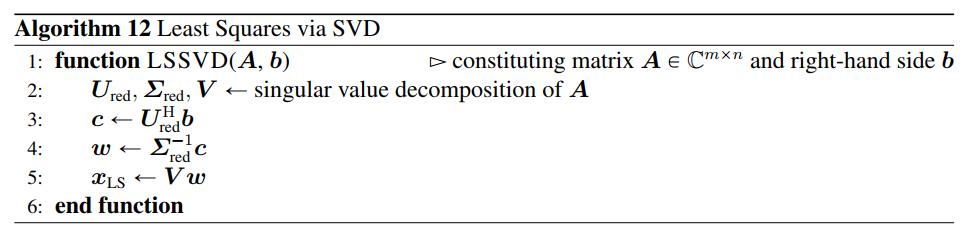
\includegraphics[width=\textwidth]{img/algo12_ls_with_SVD.png}\\
    \textbf{Operation Count Algorithm $12$}: \#FLOPS=$\mathcal{O}(2mn^2+11n^3)$
\end{sectionbox}
\begin{sectionbox}
    \subsection{Comparsion of Different Approaches}
    \begin{emphbox}
        \large \#FLOPS$_{\text{Cholesky}} \leq$\#FLOPS$_{\text{QR-Householder}}\leq$\#FLOPS$_{\text{SVD}}$
    \end{emphbox}
    The left inequality becomes and equality for $m=n$ and the right inequality is approximately an equality for $m\gg n$.\\
    For numerical stability, the order is the same
    \begin{emphbox}
        \large stability$_{\text{Cholesky}} \leq$ stability$_{\text{QR-Householder}}\leq$ stability$_{\text{SVD}}$
    \end{emphbox}
    Due to the \textbf{explicit computation of the Gram matrix} $\mathbf{A}^\text{H}\mathbf{A}$ in the Cholesky factorization based approach the condition of the problem is deteriorated considerably.\\
    QR decomposition does no perform this step. However, the \textbf{back substitution} is disadvantageous compared to the \textbf{simple scaling} and the multiplication by the unitary $\mathbf{V}$ in the SVD approach.
\end{sectionbox}
\begin{sectionbox}
    \subsection{Rank-Deficient Least Square}
    The SVD of rank-deficient $A$ is given by
    $$\mathbf{A} = \mathbf{U}_{\text{red}}\mathbf{\Sigma}_{\text{red}}\mathbf{V}^\text{H}_{\text{red}}$$
    with $\mathbf{U}_{\text{red}}\in\mathbb{C}^{m\times r}$, $\mathbf{\Sigma}_{\text{red}}\in\mathbb{C}^{r \times r}$ which is diagonal with positive diagonal elements, sub unitary $\mathbf{V}_{\text{red}} \in \mathbb{C}^{n \times r}$ and $r=$rank$(\mathbf{A})$.
\end{sectionbox}
\begin{sectionbox}
    $$\mathbf{\Sigma}^2_{\text{red}}\mathbf{V}^\text{H}_{\text{red}}\mathbf{x} = \mathbf{\Sigma}_{\text{red}}\mathbf{U}^\text{H}_{\text{red}}$$

    The equation is underdetermined with more unknowns $n$ than equations $r$. There fore infinitely many solutions for $\mathbf{x}$ exist. We rewrite the equation with

    $$\mathbf{x}_{\text{LS}} =\text{argmin}_\mathbf{x} \parallel \mathbf{x}\parallel^2_2 \quad \text{s.t.} \mathbf{\Sigma}_{\text{red}}\mathbf{V}^H_{\text{red}}\mathbf{x} = \mathbf{U}^\text{H}_{\text{red}}\mathbf{b}$$

    For rank-deficient LS we obtain the solution:
    $$\mathbf{x}_{\text{LS}}=\mathbf{V}_{\text{red}}\mathbf{\Sigma}^{-1}_{\text{red}}\mathbf{U}_{\text{red}}\mathbf{b}$$

    The residual is given by $$\mathbf{r} = (\mathbf{I} - \mathbf{U}_{\text{red}}\mathbf{U}_{\text{red}}^\text{H})\mathbf{b}$$
    that is, the residual of the rank-deficient LS problem is equal to the part of the right-hand side $\mathbf{b}$ lying in the orthogonal complment of range$(\mathbf{U}_{\text{red}})$ = range$(\mathbf{A})$.
\end{sectionbox}
\begin{sectionbox}
    \subsection{Moore-Penrose Pseudoinverse}
    The generalization for all LS problems is given by the Moore-Penrose pseudoinverse with $\mathbf{\Sigma}^\dagger = [\Sigma^\dagger_1, \mathbf{0}]$ we can rewrite $\mathbf{A}^\dagger$ as

    $$\mathbf{A}^\dagger = \mathbf{V}[\text{diag}(\frac{1}{\sigma_1}, \cdots, \frac{1}{\sigma_r}, 0, \cdots,0),\mathbf{0}]\mathbf{U}^\text{H}$$

    When $\mathbf{A}$ is full-rank and square $\mathbf{A}^\dagger = \mathbf{A}^{-1}$\\
    For full-rank and tall $\mathbf{A}\in\mathbb{C}^{m\times n}$, $m > n$: $\mathbf{A}^\dagger = (\mathbf{A}^\text{H}\mathbf{A})^{-1}\mathbf{A}^\text{H}$\\
    For full-rank and wide matrix $\mathbf{A} \in\mathbb{C}^{m\times n}$, $m < n$:\\
    $\mathbf{A}^\dagger = \mathbf{A}^H(\mathbf{A}\mathbf{A}^\text{H})^{-1}$
\end{sectionbox}
\begin{sectionbox}
    \subsection{Rank-Revealing QR Decomposition}
    The application of the rank-revealing QR decomposition of $\mathbf{A}\in\mathbb{C}^{m\times n}$ with $m\geq n$ gives
    $$\mathbf{A}\mathbf{\Pi} = \mathbf{Q}_\text{red} \mathbf{R}_\text{red}$$
    where $\mathbf{Q}_\text{red}\in\mathbb{C}^{m\times n}$ is sub unitary and

    $$\mathbf{R}_\text{red} = \begin{bmatrix}
            \mathbf{R}_{11} & \mathbf{R}_{12} \\
            \mathbf{0}      & \mathbf{0}
        \end{bmatrix}\in\mathbb{C}^{n\times n}$$
    The partition $\mathbf{R}_{11}\in \mathbb{C}^{r\times r}$ is upper-triangular and full-rank with $r$=rank$(\mathbf{A})$\\
    In every step the \textbf{column} whose lower part, that has not yet been brought to triangular form and \textbf{exhibits maximum norm} in the current step is \textbf{permuted} to the first column of the part that has not yet been transformed to triangular form.
\end{sectionbox}
\section{Condition of a Problem}
\begin{sectionbox}
    \subsection{Norm-Wise Condition Number}
    In abstract form, when solving a problem e.g., solving an equation system, the following map must be applied
    $$\mathbf{f}:\mathbb{C}^m \to \mathbb{C}^n; \mathbf{x}\to\mathbf{y}=\mathbf{f}(\mathbf{x})$$
    A prominent example for such a problem is solving an equation system of the form
    $$\mathbf{A}\mathbf{v} = \mathbf{b}$$
    Interpreting the matrix $\mathbf{A}$ constituting the equation system as parameter of the problem, the problem to be solved is:
    $$\mathbf{f}:\mathbb{C}^m \to \mathbb{C}^n; \mathbf{b}\to\mathbf{v}=\mathbf{f}(\mathbf{b})$$
    Note that a different $\mathbf{A}_2$ leads to a different problem $\mathbf{f}_2$.
\end{sectionbox}

\begin{sectionbox}
    The norm-wise condition number is given by:

    $$\kappa_\text{N}(\mathbf{f}, \mathbf{x}) = \frac{\parallel \mathbf{J}(\mathbf{x})\parallel \cdot \parallel \mathbf{x} \parallel}{\parallel \mathbf{f}(\mathbf{x})\parallel}$$

    where
    $$\mathbf{J}(\mathbf{x}) = \frac{\partial \mathbf{f}(\mathbf{x})}{\partial\mathbf{x}^T}$$

    The perturbed outcome of the problem $\mathbf{f}$ can be bouned as follows
    $$\frac{\parallel \mathbf{f}(\mathbf{x}+\Delta \mathbf{x}) - \mathbf{f}(\mathbf{x})\parallel}{\parallel \mathbf{f}(\mathbf{x})\parallel} \leq \kappa_\text{N}(\mathbf{f}, \mathbf{x}) \frac{\parallel\Delta \mathbf{x} \parallel}{\parallel \mathbf{x}\parallel} + o(\parallel \Delta \mathbf{x} \parallel)$$
    \begin{itemize}
        \item \textbf{well-conditioned}: If $\kappa_\text{N}(\mathbf{f}, \mathbf{x}) \approx 1$, (e.g., $1$,$100$). For a well-conditioned problem, it is possible fo find algorithms with small errors.
        \item \textbf{ill-conditioned}: If $\kappa_\text{N}(\mathbf{f}, \mathbf{x}) \gg 1$, (e.g., $10^6$, $10^10$). When the problem is ill-conditioned, large errors must be expected from all algorithms.
        \item \textbf{ill-posed}: If $\kappa_\text{N}(\mathbf{f}, \mathbf{x}) = \infty$. In this case, the solution $\mathbf{f}(\mathbf{x})$ either does not exist or is not unique. It can be expected that no algorithm is able so give a reasonable result.
    \end{itemize}
\end{sectionbox}
\begin{sectionbox}
    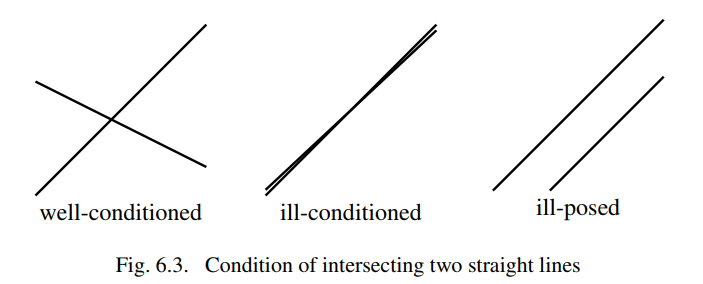
\includegraphics[width=\textwidth]{img/conditions_graphics.png}
\end{sectionbox}
\begin{sectionbox}
    \begin{tablebox}{@{\hspace{0mm}}l@{\extracolsep\fill}|l@{\extracolsep\fill}|l@{\extracolsep\fill}}
        $f(x)$ & $J(x)$ & $\kappa_\text{N}$ \\ \cmrule
        $f(x) = \sqrt{x}$ & $J(x) = \frac{d\sqrt{x}}{dx} = \frac{1}{2}\frac{1}{\sqrt{x}}$ & $\kappa_\text{N} = \frac{1}{2}$\\
        $f(x) = ax$ & $J(x)=a$& $\kappa_\text{N}=\frac{|a||x|}{|ax|}=1$\\
        $f(\begin{bmatrix}
                x_1 \\
                x_2
            \end{bmatrix})=x_1 \cdot x_2$ & $J(\mathbf{x}) = [x_2, x_1] $ & $\kappa_\text{N} = \left|\frac{x_1}{x_2}\right| + \left|\frac{x_2}{x_1}\right|$
    \end{tablebox}
\end{sectionbox}

\begin{sectionbox}
    \subsection{Component-wise Condition Number}
    The component-wise condition number is defined by
    $$\kappa_\text{C}(f,\mathbf{x}) = \frac{\parallel\mathbf{J}(\mathbf{x})\odot\mathbf{x}^\text{T}\parallel_\infty}{|f(\mathbf{x})|}$$
    $$=\frac{|\mathbf{J^\text{T}(\mathbf{x})}||\mathbf{x}| }{|f(\mathbf{x})| }$$

    the product $|\mathbf{J^\text{T}(\mathbf{x})}||\mathbf{x}|$ is performed  element wise.\\

    The component-wise condition number is smaller than the norm-wise condition number if the infinity norm is employed. For $f:\mathbb{R}^m \to \mathbb{R}$ and when applying the infinity norm, the norm wise condition number is given by
    $$\kappa_\text{N}(\mathbf{f}, \mathbf{x}) = \frac{\parallel \mathbf{J}(\mathbf{x})\parallel_\infty \cdot \parallel \mathbf{x} \parallel_\infty}{| \mathbf{f}(\mathbf{x})|}$$

    as $f(\mathbf{x})$ is assumed to be scalar. Because $\mathbf{J}^\text{T}(\mathbf{x})\in\mathbb{R}^{1\times m}$ is a row vector for scalar $f(\mathbf{x})$, $\parallel\mathbf{J}^\text{T}(\mathbf{x})\parallel_\infty = \parallel \mathbf{J}(\mathbf{x})\parallel_1 = \sum_{i=1}^{m} \left|[\mathbf{J}(\mathbf{x})]_i\right|$ holds, and due to $\parallel \mathbf{x}\parallel_\infty = $max$_{i\in\{1,\cdots,m\}}|x_i|$\\

    $$\kappa_\text{N}(f,\mathbf{x}) \geq \frac{|\mathbf{J}^\text{T}(\mathbf{x})|\cdot |\mathbf{x}|}{\left|f(\mathbf{x})\right|}=\kappa_\text{C}(f,\mathbf{x})$$

\end{sectionbox}
\begin{sectionbox}
    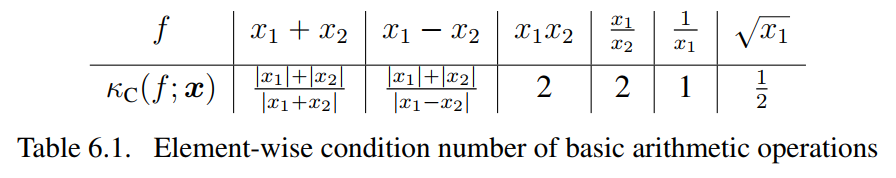
\includegraphics[width=\textwidth]{img/kc_operations.png}
\end{sectionbox}
\begin{sectionbox}
    \subsection{Condition of a Matrix}
    We can express the condition number of matrix $\mathbf{A}\in\mathbb{C}^{m \times n}$ with the help of the pseudoinverse $\mathbf{A}^\dagger$ as
    $$\kappa(\mathbf{A}) = \parallel\mathbf{A}\parallel\cdot\parallel \mathbf{A}^\dagger\parallel$$

    When we employ the $2$-norm we get the result
    $$\kappa_2(\mathbf{A}) = \parallel\mathbf{A}\parallel\cdot\parallel \mathbf{A}^\dagger\parallel = \frac{\sigma_1}{\sigma_n}$$

    \textbf{Wide Matrix}
    For a wide matrix we divide the vector $\mathbf{x}$ into a component $\mathbf{x}^\perp_\mathbf{A}$ in the nullspace of $\mathbf{A}$ and a component $\mathbf{x}_\mathbf{A}$ perpendicular to the nullspace of $\mathbf{A}$ by employing the project $\mathbf{P}_\mathbf{A}$ onto the range of $\mathbf{A}^\text{H}$, that is, $\mathbf{x}^\perp_\mathbf{A} = \mathbf{P}^\perp_\mathbf{A}\mathbf{x}$ and $\mathbf{x}_\mathbf{A} = \mathbf{P}_\mathbf{A}\mathbf{x}$, respectively, such that $\mathbf{x}^\text{H}_\mathbf{A}\mathbf{x}_\mathbf{A} = 0$. Substituting into $\kappa_\text{N}$ results in

    $$\kappa_\text{N}(\mathbf{A}\mathbf{x}, \mathbf{x}) = \frac{\parallel\mathbf{A}\parallel\cdot\parallel\mathbf{x}_\mathbf{A} + \mathbf{x}^\perp_\mathbf{A}\parallel}{\parallel\mathbf{A}\mathbf{x}_\mathbf{A}\parallel}$$

    \subsubsection{Condition of Unitary Matrix}
    $$\kappa(\mathbf{U}) = \parallel\mathbf{U}\parallel\cdot\parallel \mathbf{U}^\text{H}\parallel = 1$$
\end{sectionbox}
\section{Stability of an Algorithm}
\begin{sectionbox}
    The algorithm $\mathbf{\tilde{f}}(\mathbf{x})$ to solve a problem $\mathbf{f}(\mathbf{x})$ is denoted as

    $$\mathbf{\tilde{f}}: \mathbb{C}^m \to \mathbb{C}^n; \mathbf{x}\to \tilde{\mathbf{y}} = \mathbf{\tilde{f}}$$

    \subsection{Accuracy}
    For any possible value for the input $\mathbf{x}$, the relative error of the outcome $\mathbf{\tilde{f}}(\mathbf{x})$ of the algorithm is in the order of $\epsilon_M$, which is the least error to be expected.
    $$\forall \mathbf{x}\in\mathbb{C}^{m}:\frac{\parallel \mathbf{\tilde{f}}(\mathbf{x}) -\mathbf{f}(\mathbf{x})\parallel}{\parallel\mathbf{f}(\mathbf{x}) \parallel} = \mathcal{O}(\epsilon_\text{M})$$

    \subsection{Stability}
    An algorithm $\tilde{\mathbf{f}}$ is stable, if
    $$\forall \mathbf{x} \in \mathbb{C}^{m}: \exists \mathbf{\tilde{x}} \text{ with } \frac{\parallel \mathbf{\tilde{x}} - \mathbf{x}\parallel}{\parallel \mathbf{x}\parallel} = \mathcal{O}(\epsilon_\text{M})$$
    such that
    $$\frac{\parallel \mathbf{\tilde{f}}(\mathbf{x}) -\mathbf{f}(\mathbf{\tilde{x}})\parallel}{\parallel\mathbf{f}(\mathbf{\tilde{x}}) \parallel} = \mathcal{O}(\epsilon_\text{M})$$
    \textbf{It is not possible to infer the accuracy of an algorithm from the observation that it is stable}.

    \subsection{Backward Stability}
    An algorithm $\tilde{\mathbf{f}}$ is backward stable, if
    $$\forall \mathbf{x} \in \mathbb{C}^{m}: \exists \mathbf{\tilde{x}} \text{ with } \frac{\parallel \mathbf{\tilde{x}} - \mathbf{x}\parallel}{\parallel \mathbf{x}\parallel} = \mathcal{O}(\epsilon_\text{M})$$
    such that
    $$\tilde{\mathbf{f}}(\mathbf{x}) = \mathbf{f}(\tilde{\mathbf{x}})$$

    This definition of backward stability is stronger than the definition of stability before, since the relative error between the output of the algorithm for the true input $\mathbf{x}$, i.e., $\tilde{\mathbf{f}}(\mathbf{x})$, and the output of the underlying problem $\mathbf{f}(\tilde{\mathbf{x}})$ for the perturbed input $\tilde{\mathbf{x}}$ most be zero. \textbf{Backward stability implies stability}.

    $$\frac{\parallel \mathbf{\tilde{f}}(\mathbf{x}) -\mathbf{f}(\mathbf{x})\parallel}{\parallel\mathbf{f}(\mathbf{x}) \parallel} = \mathcal{O}(\kappa_\text{N}(\mathbf{f},\mathbf{x})\epsilon_\text{M})$$
\end{sectionbox}

\section{System of Equations}
\begin{sectionbox}
    $$\mathbf{A} = \mathbf{L}\mathbf{U}$$
    with the unit lower-triangular $\mathbf{L} \in\mathbb{C}^{m\times m}$ and the upper-triangular $\mathbf{U}\in\mathbb{C}^{m\times m}$
    The coefficients for $\mathbf{L}$ are given as  $l_{i,j} = \frac{a_{ij}}{ajj}$

    $$\mathbf{L} = \mathbf{I}+\mathbf{l}_1\mathbf{e}^\text{T}_1+\cdots\mathbf{l}_{m-1}e^\text{T}_{m-1}$$
    $$=\begin{bmatrix}
            1       &        &           &   & \\
            l_{21}  & 1      &           &   & \\
            \vdots  & \ddots & \ddots    &   & \\
            l_{m,1} & \cdots & l_{m,m-1} & 1
        \end{bmatrix}$$

\end{sectionbox}
\begin{sectionbox}
    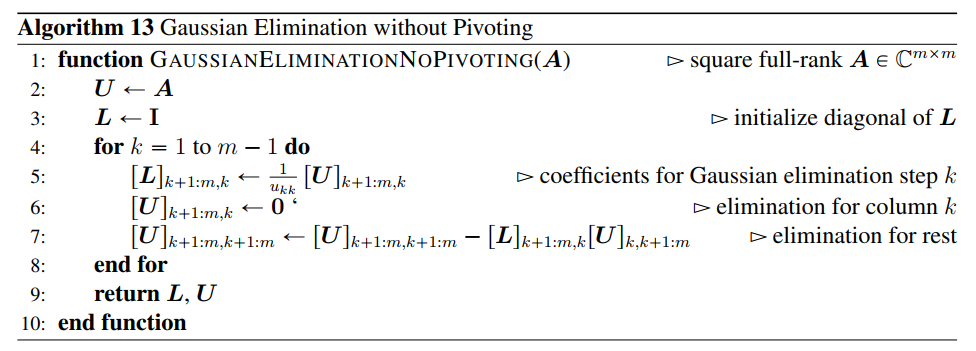
\includegraphics[width=\textwidth]{img/algo13_gauss_without_pivo.png}
    \textbf{Operation Count Algorithm $13$}: \#FLOPS=$\mathcal{O}(\frac{2m^3}{3})$

\end{sectionbox}
\begin{sectionbox}
    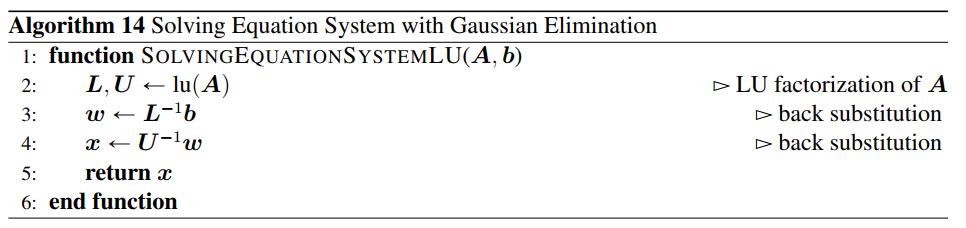
\includegraphics[width=\textwidth]{img/algo14_solve_with_gauss.png}
    \textbf{Operation Count Algorithm $14$}: \#FLOPS=$\mathcal{O}(\frac{2m^3}{3} + 2n^2)$\\
    Worst case error for Gauss with LU is:\\
    $\mathcal{O}(\rho_{\text{worst-case}} \cdot \epsilon_\text{M})$ with $\rho_{\text{worst-case}} = 2^{m-1}$. Solving an equation system with QR does not have such problems.
\end{sectionbox}
\begin{sectionbox}
    \begin{sectionbox}
        \subsection{Stability of Gaussian Elimination}
        Without pivoting it holds that
        $$\tilde{\mathbf{L}}\tilde{\mathbf{U}} = \mathbf{A} + \Delta\mathbf{A}\quad \text{ with } \frac{\parallel \Delta \mathbf{A} \parallel}{\parallel\mathbf{L}\parallel\parallel\mathbf{U}\parallel} = \mathcal{O}(\epsilon_\text{M})$$
        \textbf{Gaussian elimination without pivoting is not backward stable!}
    \end{sectionbox}
    \subsection{Complete Pivoting}
    Leads to smallest coefficients for back substitution procedure. We have to compare $(m-k+1)^2$ elements in the $k$-th step. All entries in $\mathbf{L}$ below the diagonal are smaller than one.
    \begin{emphbox}
        \large \textbf{Operation Count}: \#FLOPS=$\mathcal{O}(\frac{m^3}{3})$\\
    \end{emphbox}
    Full pivoting ensures that all off-diagonal elements of the resulting $\mathbf{U}$ are smaller than or equal to the diagonal entry in the same row. Thus complete pivoting also improves the properties of the second back substitution.
\end{sectionbox}
\begin{sectionbox}
    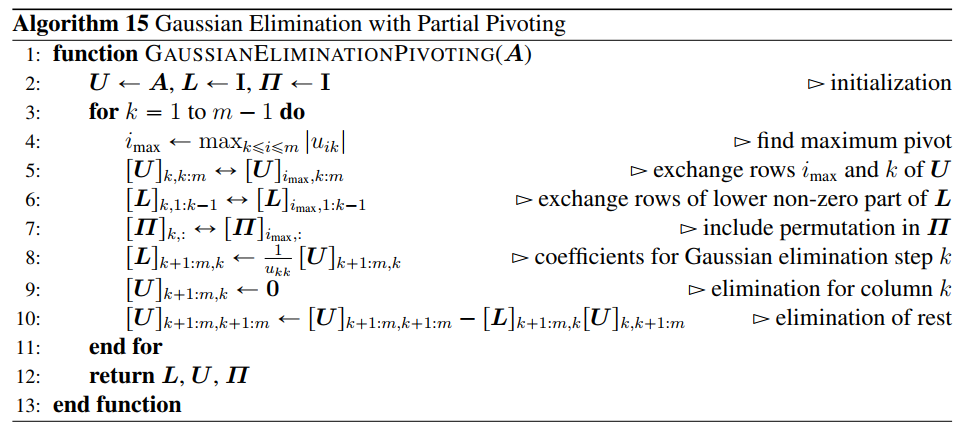
\includegraphics[width=\textwidth]{img/algo15_gauss_partial_pivoting.png}
    \textbf{Operation Count Algorithm $15$}: \#FLOPS=$\mathcal{O}(\frac{2m^3}{3} + \frac{m^2}{2})$\\
\end{sectionbox}
\begin{sectionbox}
    \subsection{Partial Pivoting}
    With partial pivoting we have
    $$\mathbf{\Pi}\mathbf{A} = \mathbf{L}\mathbf{U}$$
    For partial pivoting $m-k+1$ elements must be compared in step $k$
    \begin{emphbox}
        \large \textbf{Operation Count}: \#FLOPS=$\mathcal{O}(\frac{m^2}{2})$\\
    \end{emphbox}
    The computational costs of partial pivoting compared to the LU factorization ($\mathcal{O}(\frac{2m^3}{3})$) are neglectable.
    \begin{emphbox}
        \large Gaussian elimination with partial pivoting is potentially backward stable. With growth factor $\rho=\frac{\text{max}_{i,j}(|u_{i,j}|)}{\text{max}_{i,j} |a_{i,j}|}$
    \end{emphbox}
    With pivoting it holds:
    $\tilde{\mathbf{L}}\tilde{\mathbf{U}} = \mathbf{A} + \Delta\mathbf{A}\quad \text{ with } \frac{\parallel \Delta \mathbf{A} \parallel}{\parallel\mathbf{L}\parallel\parallel\mathbf{U}\parallel} = \mathcal{O}(\rho \epsilon_\text{M})$
\end{sectionbox}
\begin{sectionbox}
    \subsection{Cholesky Factorization}
    A positive definite matrix $\mathbf{A}$ is Hermitian i.e. $\mathbf{A}^\text{H} = \mathbf{A}$
    All eigenvalues of a Hermitian $\mathbf{A}$ are real-valued. If $\mathbf{A}$ is not only Hermitian but positive definite, all eigenvalues are not only real-valued but also positive!
    $$\forall \mathbf{x}\in\mathbb{C}^{m}: \mathbf{x}^\text{H}\mathbf{A}\mathbf{x} > 0$$

    $$\mathbf{A} \succ 0$$

    \begin{emphbox}
        \large For Cholesky the matrix $\mathbf{A}$ must be positive definite!\\ $\mathbf{A} \succ 0$
    \end{emphbox}
    \textbf{All diagonal elements of a positive definite matrix are greater than zero!}
    $$\mathbf{e}^\text{T}_k \mathbf{A}\mathbf{e}^\text{T}_k = [\mathbf{A}]_{k,k} > 0$$
    With the Cholesky factorization the root of matrix can be defined as
    $$\mathbf{A}^{1/2} = \mathbf{L}\mathbf{D}^{1/2}$$
    $$\mathbf{A} = \mathbf{A}^{1/2}\mathbf{A}^{\text{H}/2}$$

\end{sectionbox}
\begin{sectionbox}
    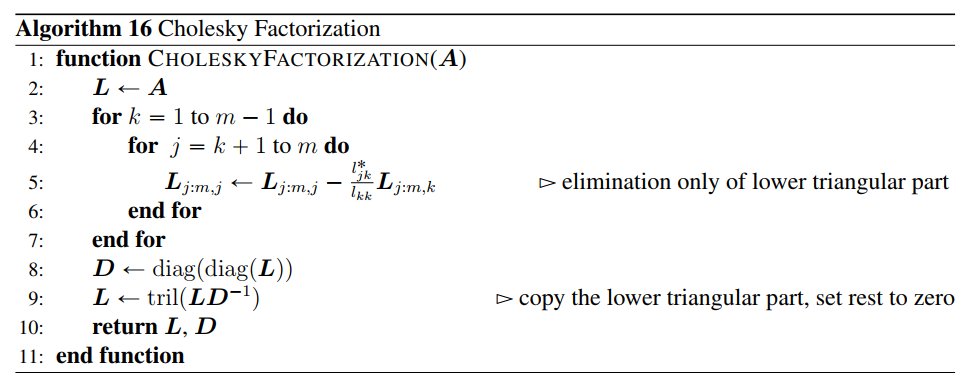
\includegraphics[width=\textwidth]{img/algo16_cholesky.png}
    \textbf{Operation Count Algorithm $16$}: \#FLOPS=$\mathcal{O}(\frac{1}{3}m^3)$\\
    \#FLOP$_k = \sum_{j=k+1}^{m} 2m-2j+3 = \sum_{j'=1}^{m-k}2j'+1$\\
    $=(m-k)(m-k+1)+m-k\approx m^2-2mk+k^2$\\

    \#FLOPS$=\sum_{k=1}^{m-1}\text{\#FLOPS}_k = \sum_{k=1}^{m-1}m^2-2mk+k^2$\\
    $=(m-1)m^2-m^2(m-1)+\frac{(2m-1)m(m-1)}{6}$
\end{sectionbox}
\begin{sectionbox}
    \subsection{Stability of Cholesky Factorization}
    Contrary to Gaussian Elimination, the Cholesky factorization can be used without pivoting. If, however, the stability of the Cholesky factorization must be improved, pivoting can be employed.
    $$\mathbf{\Pi}\mathbf{A}\mathbf{\Pi}^\text{T} = \mathbf{L}\mathbf{D}\mathbf{L}^\text{H}$$
    \begin{emphbox}
        \large Cholesky factorization, even without pivoting, can be shown to be backward stable
    \end{emphbox}
\end{sectionbox}
\begin{sectionbox}
    \subsection{Hessenberg-Form}
    A matrix whose elements below the first lower sub-diagonal are all zero is called \textbf{Hessenberg} matrix $\mathbf{H}$
    $$\mathbf{Q}^\text{H}\mathbf{A}\mathbf{Q} = \begin{bmatrix}
            \times & \times & \cdots & \times & \times \\
            \times & \times & \cdots & \times & \times \\
            0      & \times & \cdots & \times & \times \\
            \vdots & \ddots & \ddots & \vdots & \vdots \\
            0      & \cdots & 0      & \times & \times \\
        \end{bmatrix}$$

    The Hessenberg-Form can be achieved for a matrix $\mathbf{A}\in\mathbb{C}^{m\times m}$if we employ unitary reflection matrices $\mathbf{Q}_i$ with the resulting reflection matrix $\mathbf{Q}=\mathbf{Q}_1\cdots\mathbf{Q}_{m-2}$.
    $$\mathbf{Q} = \begin{bmatrix}
            \mathbf{I}_i & \mathbf{0}^\text{T} \\
            \mathbf{0}   & \mathbf{F}_i
        \end{bmatrix} \in \mathbb{C}^{m\times m}$$
    With the Householder reflectors $\mathbf{F}_i\in\mathbb{C}^{m-i+1\times m-i+1}$ and\\
    $I_i\in\mathbb{C}^{i-1\times i-1}$\\

    For Hermitian $\mathbf{A}$, i.e. $\mathbf{A}^\text{H}=\mathbf{A}$ the result of the transformations leading to a Hessenberg matrix is a Hermitian Hessenberg matrix, that is, a tri-diagonal matrix.
    $$\mathbf{H} = \mathbf{Q}^\text{H} \mathbf{A}\mathbf{Q}=
        \begin{bmatrix}
            \times & \times & 0      & 0      & 0      & \cdots & 0      \\
            \times & \times & \times & 0      & 0      & \cdots & 0      \\
            0      & \times & \times & \times & 0      & \cdots & 0      \\
            \vdots & \ddots & \ddots & \ddots & \ddots & \ddots & \vdots \\
            0      & \cdots & 0      & \times & \times & \times & 0      \\
            0      & \cdots & 0      & 0      & \times & \times & \times \\
            0      & \cdots & 0      & 0      & 0      & \times & \times \\
        \end{bmatrix} = \mathbf{H}^\text{H}$$
\end{sectionbox}
% ======================================================================
% End
% ======================================================================
\end{document}
